\subsection{Full protocol: the federated failure comes from unscaled inputs}\label{sec:full}

Fig.~\ref{fig:regimes} shows the per-dimension audit on the pooled test set for the baseline and the full protocol. The full protocol lifts FedAvg's macro-AUC from 0.518 to 0.643 and moves every dimension above chance (Sleep 0.497 $\rightarrow$ 0.613, Mental 0.505 $\rightarrow$ 0.643, Wellbeing 0.488 $\rightarrow$ 0.706). An ablation on seeds 42, 123 and 456 attributes the whole gain to preprocessing: standardized inputs with one-hot race/ethnicity reach 0.639 even with the baseline learning rate and the final round, whereas validation-based checkpoints and the tuned learning rate on raw inputs reach only 0.517. In the baseline, FedAvg trained on unscaled inputs (ages near 50, blood pressure near 120, category codes 1--7) whose distributions differ across clients; centralized training tolerated this and federated averaging did not. With standardized inputs, federation costs 0.008 macro-AUC (95\% CI [0.006, 0.010], lower on all 10 seeds, Holm $p<10^{-3}$; at most 0.013 on any dimension) and no dimension falls to chance. Richer features raise macro-AUC to 0.697 (C1) and 0.689 (C3), most for Mental, Metabolic and Wellbeing (+0.07 to +0.09).

The other aggregation schemes behave as follows (Table~\ref{tab:summary}). Standard SCAFFOLD closes the remaining gap (macro-AUC $+0.007$ over FedAvg with both feature sets, Holm $p<10^{-3}$, level with C1); Ditto's personalized models with the tuned $\lambda{=}1$ add 0.004 (Holm $p \leq 0.01$); and CS-Agg, q-FedAvg, FedProx and C8 stay within 0.003 of FedAvg. The per-dimension audit did its job: it exposed a preprocessing problem that neither the composite score nor per-client MG could reveal.

\begin{figure*}[t]
\centering
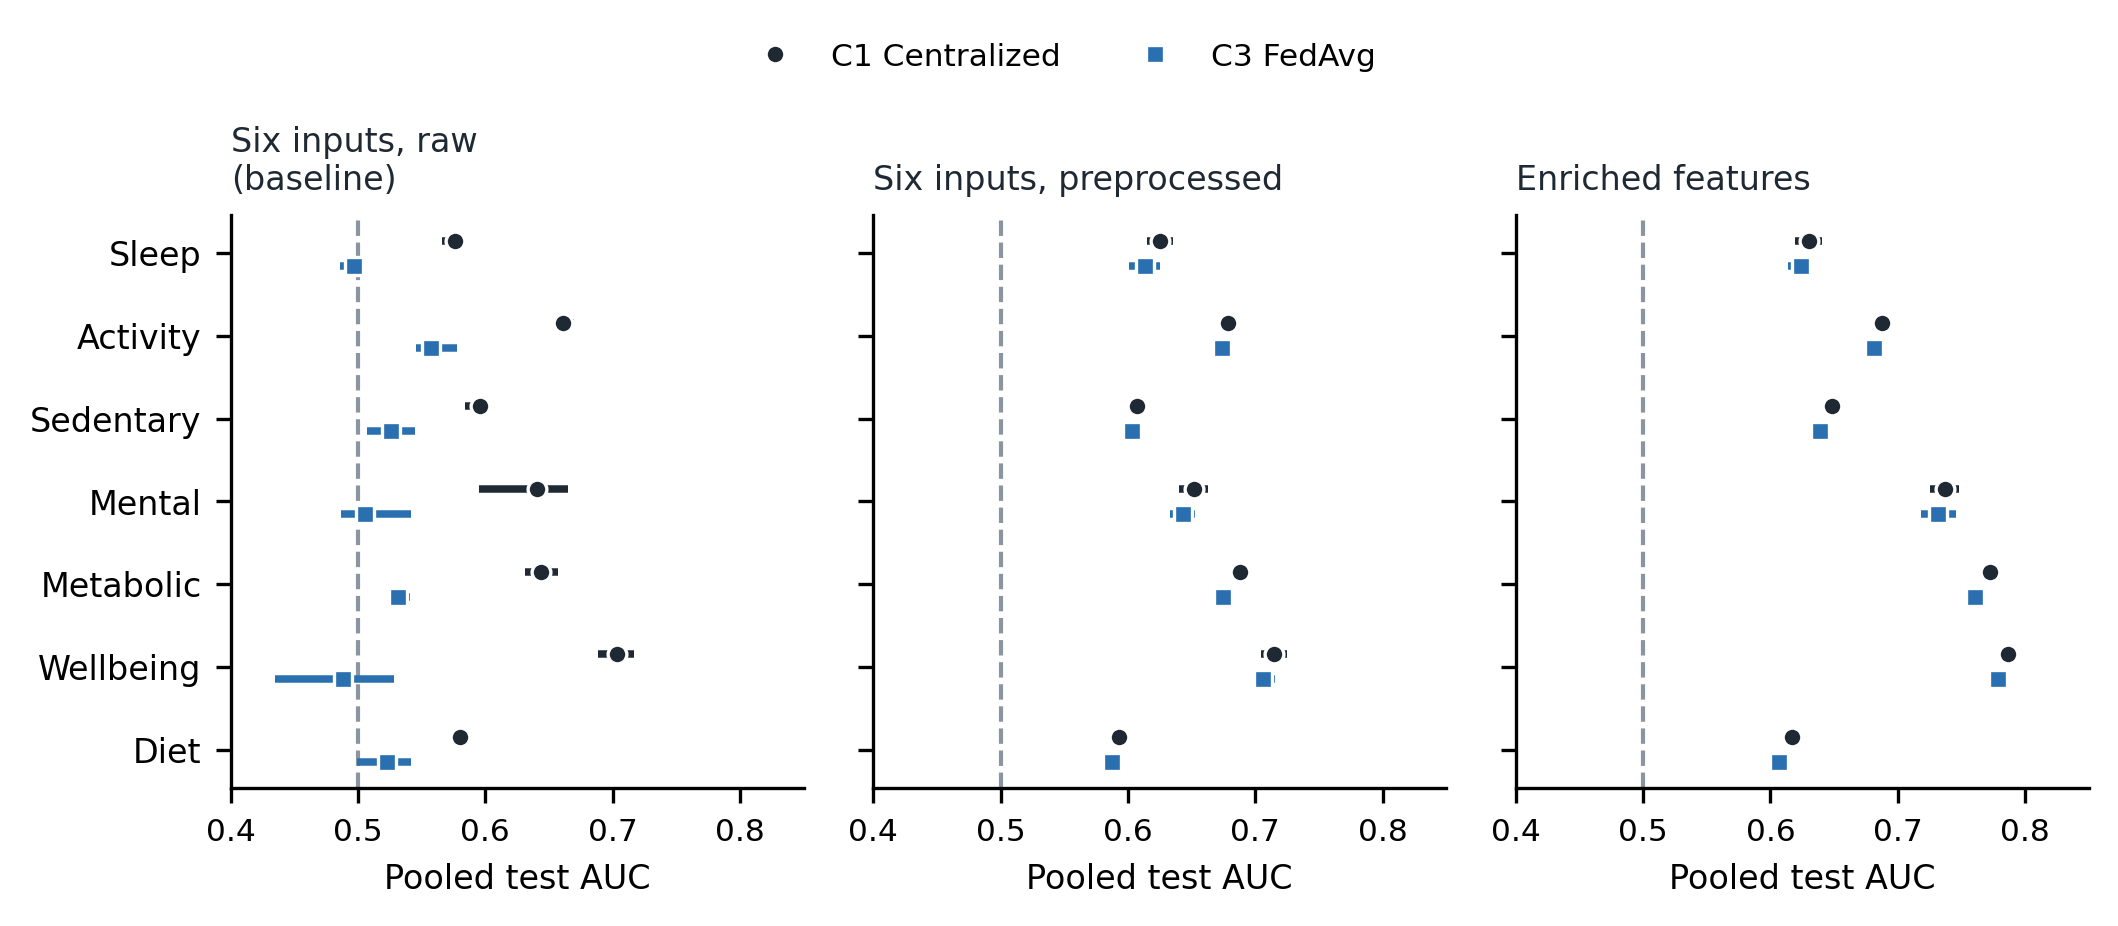
\includegraphics[width=0.86\textwidth]{fig13_dimension_auc_by_regime.png}
\caption{Pooled test AUC per dimension (mean and 95\% CI over seeds) for centralized (C1) and FedAvg (C3) training: the baseline with raw inputs (3 seeds), and the full protocol with the six base inputs preprocessed and with the enriched feature set (10 seeds each). Dashed: chance.}
\label{fig:regimes}
\end{figure*}

\begin{table}[t]
\caption{Summary of the baseline and full protocol (pooled test set, mean over seeds). Macro: AUC averaged over dimensions. Min: worst dimension's AUC. Pooled MG: its chance 95th percentile is about 0.04. MG-exc.: per-client MG minus its label-permutation null ($^{*}$ Holm $p<0.05$ across all 30 conditions analyzed, clients as units). $\bar\Delta$: blind spot averaged over dimensions. ECE: expected calibration error.}
\label{tab:summary}
\centering\small
\setlength{\tabcolsep}{2.6pt}
\begin{tabular}{@{}lcccccc@{}}
\toprule
Condition & Macro & Min & Pooled MG & MG-exc. & $\bar\Delta$ & ECE \\
\midrule
\multicolumn{7}{@{}l}{\emph{Baseline (six raw inputs, 3 seeds)}} \\
C1 & 0.629 & 0.574 & 0.055 & $+0.004$ & 0.063 & 0.032 \\
C3 FedAvg & 0.518 & 0.469 & 0.049 & $+0.013$ & 0.037 & 0.039 \\
\multicolumn{7}{@{}l}{\emph{Full protocol, six inputs preprocessed (10 seeds)}} \\
C1 & 0.651 & 0.592 & 0.059 & $+0.010$ & 0.070 & 0.020 \\
C2 & 0.650 & 0.591 & 0.059 & $+0.010$ & 0.069 & 0.021 \\
C3 FedAvg & 0.643 & 0.586 & 0.058 & $+0.011$ & 0.067 & 0.024 \\
C2-FL & 0.644 & 0.584 & 0.060 & $+0.012$ & 0.068 & 0.026 \\
C4 SCAFFOLD & 0.651 & 0.593 & 0.058 & $+0.007$ & 0.069 & 0.022 \\
C5 CS-Agg & 0.643 & 0.584 & 0.059 & $+0.009$ & 0.066 & 0.024 \\
C6 Ditto & 0.647 & 0.588 & 0.060 & $+0.009$ & 0.068 & 0.021 \\
C7 q-FedAvg & 0.642 & 0.585 & 0.057 & $+0.009$ & 0.065 & 0.024 \\
C8 & 0.643 & 0.586 & 0.057 & $+0.010$ & 0.068 & 0.023 \\
C9 FedProx & 0.644 & 0.585 & 0.059 & $+0.010$ & 0.067 & 0.028 \\
C3 + class wt. & 0.627 & 0.574 & 0.053 & $+0.008$ & 0.053 & 0.170 \\
C3 + focal & 0.641 & 0.582 & 0.059 & $+0.011^{*}$ & 0.064 & 0.108 \\
\multicolumn{7}{@{}l}{\emph{Full protocol, enriched features (10 seeds)}} \\
C1 & 0.697 & 0.615 & 0.083 & $+0.023^{*}$ & 0.078 & 0.027 \\
C2 & 0.695 & 0.612 & 0.083 & $+0.024^{*}$ & 0.076 & 0.030 \\
C3 FedAvg & 0.689 & 0.604 & 0.084 & $+0.024^{*}$ & 0.073 & 0.023 \\
C2-FL & 0.688 & 0.607 & 0.082 & $+0.023^{*}$ & 0.073 & 0.029 \\
C4 SCAFFOLD & 0.696 & 0.611 & 0.085 & $+0.022^{*}$ & 0.077 & 0.022 \\
C5 CS-Agg & 0.688 & 0.606 & 0.083 & $+0.023^{*}$ & 0.073 & 0.031 \\
C6 Ditto & 0.692 & 0.607 & 0.086 & $+0.023^{*}$ & 0.074 & 0.028 \\
C7 q-FedAvg & 0.688 & 0.605 & 0.083 & $+0.024^{*}$ & 0.073 & 0.030 \\
C8 & 0.686 & 0.603 & 0.083 & $+0.023^{*}$ & 0.073 & 0.030 \\
C9 FedProx & 0.687 & 0.604 & 0.083 & $+0.023^{*}$ & 0.073 & 0.030 \\
C3 + class wt. & 0.674 & 0.601 & 0.074 & $+0.024^{*}$ & 0.060 & 0.144 \\
C3 + focal & 0.686 & 0.601 & 0.084 & $+0.023^{*}$ & 0.070 & 0.111 \\
\bottomrule
\end{tabular}
\end{table}

\subsection{Per-client masking grows with signal but stays small}

Table~\ref{tab:summary} shows how per-client MG changes as the models improve. With the six preprocessed inputs, MG-excess is $+0.007$ to $+0.012$, and only C3 with focal loss differs from chance after Holm correction ($p=0.037$). With richer features, the dimensions separate more (pooled MG about 0.08, against a chance 95th percentile of about 0.04), and an excess of $+0.022$ to $+0.024$ appears in every condition (Holm $p \leq 0.001$; 9.0--13.5\% of client results above the null 95th percentile). Even so, this real excess is about a fifth of the raw per-client MG (0.12--0.13); the rest is noise. A calibrated statistic shows this dose--response; raw MG cannot, since it stays at 0.11--0.13 in every regime.

Population-level MG exceeds its chance 95th percentile in every full-protocol configuration on average over seeds (in 90--100\% of individual seeds), centralized training included. It reflects how unevenly learnable the seven dimensions are from these inputs, not something federated training causes. Whether the composite \emph{hides} that unevenness is a separate question, answered in Section~\ref{sec:blind}.

\emph{Other partitions.} The results do not depend on the income-by-age clients. With a random split into 20 equal clients (65--109 test records each), raw MG is 0.11--0.13 against a chance level of 0.100, and MG-excess is $+0.011$ (six inputs) and $+0.024$ to $+0.025$ (enriched). With 12 race/ethnicity $\times$ sex clients (24--332 records) the excess is largest, $+0.030$ to $+0.032$ and $+0.043$, and the same for centralized predictions grouped the same way, so it reflects differences between demographic groups in the data, not federation. Under all three partitions, FedAvg stays within 0.009 macro-AUC of centralized training and $\Delta_d$ stays between 0.02 and 0.15.

\subsection{The composite score hides every dimension's signal}\label{sec:blind}

In every full-protocol configuration and every dimension, the composite flags poor cases worse than the dimension's own output: $\Delta_d$ ranges from 0.015 to 0.157 AUC, and the 95\% CIs over seeds exclude zero in all 196 configuration--dimension pairs (Fig.~\ref{fig:blind}). The loss is largest for Sedentary (0.10--0.16) and Activity (0.05--0.10) and smallest for Metabolic (0.02--0.05), and it is similar for every aggregation scheme and loss (0.06--0.07 averaged over dimensions). In the baseline FedAvg runs, $\Delta_d$ was small for Sleep, Mental, Wellbeing and Diet ($-0.016$ to $+0.029$), but only because those outputs carried little signal to hide.

\begin{figure}[t]
\centering
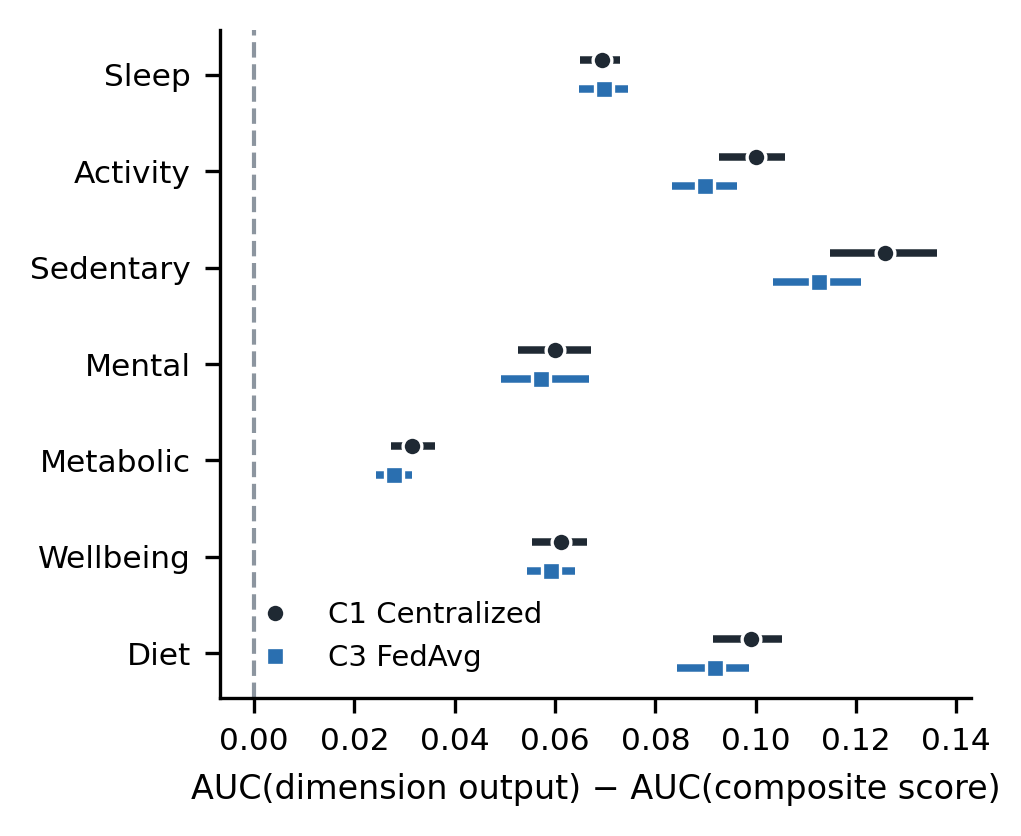
\includegraphics[width=0.92\columnwidth]{fig14_composite_blind_spot.png}
\caption{Composite blind spot $\Delta_d$ (enriched features, 10 seeds, 95\% CI): how much worse the composite score is than the dimension's own output at flagging that dimension's poor cases.}
\label{fig:blind}
\end{figure}

\subsection{Class imbalance, thresholds and decoupled training}

At the default 0.5 threshold, models trained with plain cross-entropy almost never flag Sleep (TPR 0.00--0.02) or Mental (0.00--0.03). With a threshold tuned on validation data, the same models reach TPR 0.51--0.62 for Sleep and 0.57--0.70 for Mental, and mean balanced accuracy rises from 0.55 to 0.60 (preprocessed inputs) and from 0.58 to 0.64 (enriched). Near-zero sensitivity at 0.5 is a threshold artifact, not a property of the training objective.

Class weighting moves the default operating point (Sleep TPR 0.54--0.61 at 0.5), but it lowers FedAvg macro-AUC by 0.014--0.017 (all 10 seeds) and raises ECE from about 0.02 to 0.14--0.17. Focal loss changes AUC by at most 0.004 and raises ECE to about 0.11. Training each dimension as a separate federation (C2-FL) costs seven times FedAvg's communication, yet it does not differ from FedAvg on macro-AUC, worst-dimension AUC or pooled MG in either feature set (all $|\text{difference}| \leq 0.003$, Holm $p \geq 0.81$). More broadly, no aggregation scheme or decoupled objective changes pooled MG relative to its reference; of 26 paired comparisons, only class weighting with enriched features lowers it ($-0.011$, Holm $p=0.002$), and it does so while lowering macro-AUC by 0.014 (all others $|\text{difference}| \leq 0.005$, Holm $p \geq 0.81$).

\subsection{Subgroup fairness and attribution stability}

Masking also occurs across demographic groups. Across the plain cross-entropy configurations with preprocessed inputs, the AUC gap between income groups is largest for Mental (0.15--0.20) and Wellbeing (0.10--0.12), and the worst income group's Mental AUC is at chance (0.46--0.49). Richer features narrow the Mental gap to 0.13--0.14 and raise the worst group to 0.63--0.67. One global threshold turns these gaps into large equal-opportunity violations: Mental sensitivity differs between income groups by 0.78--0.84 and Wellbeing by 0.82--0.86 (0.38--0.55 and 0.42--0.50 with richer features), because prevalence falls steeply with income. Federated and centralized training behave alike here.

\emph{Attribution stability.} We computed SHAP attributions~\cite{lundberg2017} (GradientExplainer, 100 background and 300 explained test records) for the centralized model of every seed. For multi-column feature groups such as race/ethnicity, we sum each person's signed contributions before averaging their magnitude. Group rankings agree closely across seeds (Kendall's $W$ = 0.90--0.99 with the six inputs, 0.78--0.95 with richer features), and each dimension's top group is the same in 50--100\% of seeds. Effect directions match established epidemiology in all ten seeds: a lower poverty-income ratio raises predicted risk of depression~\cite{lorant2003} and of fair/poor self-rated health~\cite{braveman2014}, older age raises risk of insufficient activity, and male sex raises risk of above-median sugar intake. With richer features, prescription count leads for Mental and cholesterol (total and HDL) for Metabolic in every seed, while education and prescription count split the lead for Wellbeing (5 vs.\ 5 of 10). A single seed can mislead: for Metabolic with the six inputs, systolic blood pressure and race/ethnicity swap the top rank across seeds (6 vs.\ 4 of 10).
